% !TeX encoding = UTF-8
% !TeX spellcheck = en_GB
% !TeX root = CircuitsCheatSheet.tex
\documentclass[]{article}

\usepackage[siunitx]{circuitikz}

%opening
\title{Circuits CheatSheet}
\author{Daniel Vilas}

\begin{document}

\maketitle

\begin{abstract}
Schematics an formulas from Coursera Courses
\end{abstract}
\section{Coursera}
\subsection{Basic Formulas}
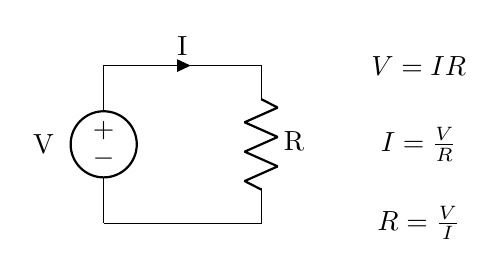
\begin{tikzpicture}[american]
\draw(0,0) to[V=V, invert] (0,2) to[short, i=I] (2,2)
to[resistor, R=R] (2,0) -- (0,0)
;
\draw (4,2) node {$V=IR$};
\draw (4,1) node {$I=\frac{V}{R}$};
\draw (4,0) node {$R=\frac{V}{I}$};
\end{tikzpicture}

Figure 1

\subsection{Module 1}
Electric current (I) is the quantity of charge (Q) coulombs that passes through a given area in a specified time (t).

$$i(t)=\frac{dQ(t)}{dt}$$
$$I=\frac{Q}{t}$$

Voltage (V) is the change in energy in joules (w) per coulomb of charge (C)

$$v=\frac{dw}{dq}$$
Charged particles (q) flow over time (t) and produce current (i).
Voltage (v) is produced by the energy (w) lost or gained by the moving charge (q).
Power (p) is the rate at which the charges’ energy (w) changes over time (t).
$$p=\frac{dw}{dt}$$
Power can also be expressed as the product of current and voltage.
$$p=\frac{dw}{dt}=\frac{dw}{dq}\cdot\frac{dq}{dt}=v\cdot i$$

Electrical resistance is determined by the material’s cross sectional area (A), length (L), and resistivity ($\rho$).
$$R=\frac{\rho L}{A}$$
Conductance (G) is the reciprocal of resistance
$$G=\frac{1}{R}=\frac{\sigma A}{L}$$
$$\sigma = \frac{1}{\rho}$$


\subsection{Module 2}
KVL: Sum of the voltages around any loop = zero. If a current enters on - the voltage is negated.
$$\sum_{i}^{loop} Vi =0 $$

KCL: Sum of the currents leaving a node = sum of current entering the node. Or the sum of all currents 0 supposing all are entering (negative after analysis means the current leaves)

$$\sum Ientering = \sum Ileaving$$

Resistors in Series

$$Req=\sum Ri$$

Resistors in Parallel

$$Req=\frac{1}{\sum\frac{1}{Ri}}$$
$$Req=\frac{R1\cdot R2}{R1+R2}$$

Voltage Divider Law. 
Two resistors in series R1 and R2, Vi=voltage across Ri:
$$Vi=\frac{Ri}{R1+R2}Vs$$

Current Divider Law. 
Two resistors in parallel R1 and R2, Ii=current flows through Ri, Rc the other resistor:
$$Ii=\frac{Rc}{R1+R2}Is$$
\subsection{Module 3}
Mesh Analysis

1. Define mesh currents, one for each noninclusive
loop
2. Do KVL around each loop
3. Solve for mesh currents

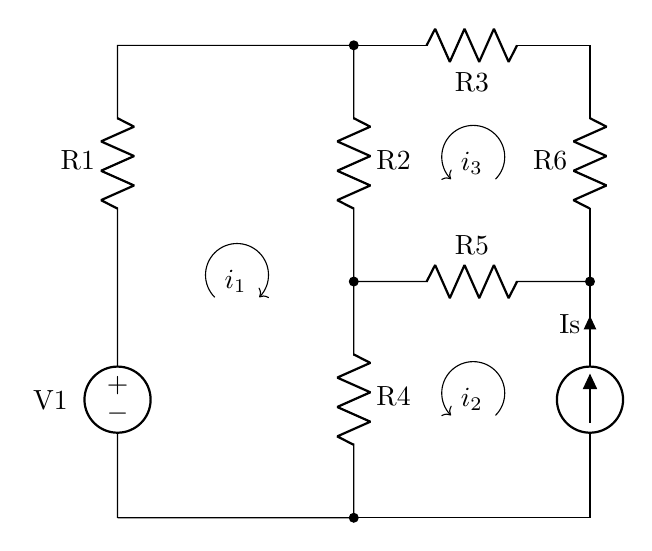
\begin{tikzpicture}[american]
\draw(0,0) to[V=V1, invert] (0,3)
          to [R=R1] (0,6)
          to [short] (3,6) 
          to [R=R2] (3,3)
          to [R=R4] (3,0)
          to [short] (0,0);
\draw(3,0) to [short, *-] (6,0)
		  to [I=Is] (6,3)
		  to [R=R6] (6,6)
		  to [R=R3, -*] (3,6);
\draw (3,3) to [R=R5, *-*] (6,3);
\draw (1.5,3) node {$i_1$};
\draw[<-] (1.8,2.8) arc (-45:225:0.4);
\draw (4.5,1.5) node {$i_2$};
\draw[->] (4.8,1.3) arc (-45:225:0.4);
\draw (4.5,4.5) node {$i_3$};
\draw[->] (4.8,4.3) arc (-45:225:0.4);
\end{tikzpicture}

From KCL:

$$-V1+R1i_1 +R2(i_1+i_3)+R3(i_1+i_3)=0$$
$$V_is+R5(i_2-i_3)+R4(i_2+i_1)=0$$
$$R6i_3+R3(i_3)+R2(i3_+i_2)+R5(i3-i_2)=0$$

Also, as Is is a current source include `$Is=i_2+i_3$'

\newpage
Node Analysis

1. Select a ground node
2. Define node voltages
3. Do KCL at nodes with unknown voltages
4. Solve for node voltages

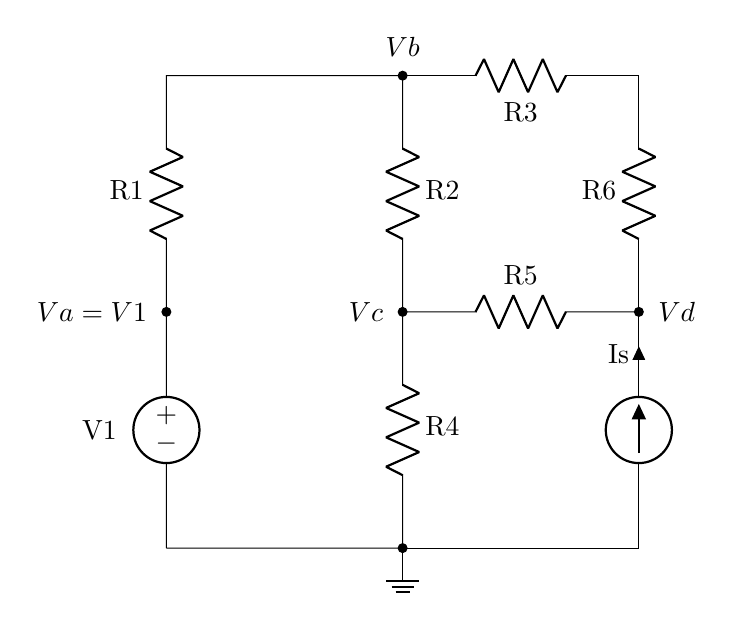
\begin{tikzpicture}[american]
\draw(0,0) to[V=V1, invert, -*] (0,3) node[label={left:$Va=V1$}] {}
to [R=R1] (0,6)
to [short] (3,6)  node[label={above:$Vb$}] {}
to [R=R2] (3,3) node[label={left:$Vc$}] {}
to [R=R4] (3,0)
to [short] (0,0);
\draw(3,0) node[ground]{} to [short, *-] (6,0)
to [I=Is] (6,3) node[label={right:$Vd$}] {}
to [R=R6] (6,6)
to [R=R3, -*] (3,6);
\draw (3,3) to [R=R5, *-*] (6,3);

\end{tikzpicture}
$$Node A := Va=V1$$
$$Node B := \frac{Vb-Va}{R1}+\frac{Vb-Vc}{R2} +\frac{Vb-Vd}{R3+R6}=0$$
$$Node C := \frac{Vc-Vb}{R2}+\frac{Vc-Vd}{R5} +\frac{Vc-0}{R4}=0$$
$$Node D := \frac{Vd-Vc}{R5}+\frac{Vd-Vb}{R3+R6} -Is=0$$

\subsection{Module 4}
Thevenin-Norton
From 2 terminals all circuits can be simplified to simple form:

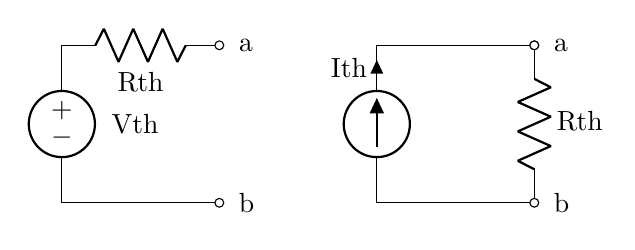
\begin{tikzpicture}[american]
\draw(2,2) node[label={right:a}] {} to[R=Rth,o-] (0,2) 
to [V=Vth] (0,0)
to [short, -o] (2,0) node[label={right:b}] {};;

\draw(6,2) node[label={right:a}] {} to[R=Rth,o-o] (6,0) node[label={right:b}] {}
to [short] (4,0)
to [I=Ith] (4,2)
to [short, -o] (6,2);
\end{tikzpicture}

$Rth$ is calculated as the $Req$ when the sources are removed (Voltage := ShortCut and Current := Break). $Vth$ is the voltage shown between nodes A and B $Vab$, Ith is the current that flows between nodes A and B if a short is placed between them.
$$Vth=Ith\cdot Rth$$

Usually those versions are for calculating the maximum power dissipated by a load $Rl$ will be $RL=Rth$
$$P=Vab\frac{Vab}{Rl}=\left(\frac{RL}{Rth+Rl}Vth\right)^2 \frac{1}{Rl}$$

When simplifying a circuit you can interchange Thevening Norton parts.

Superposition in Circuits

The voltage/current for a component could be calculated as the sum of the individual effect for each source as it is the only source.

1. Zero all sources but one, and find the
output to that source.
2. Repeat this procedure for each source.
3. Sum the corresponding outputs.

\subsection{Module 5}
Capacitors
Capacitance (C) in Farads relates to the charge (q) in Coulombs and the voltage (v) in volts, according to
$$q=Cv$$
$$C=\varepsilon\frac{A}{d}$$
$$\varepsilon=\varepsilon_r\cdot\varepsilon_0$$
$$\varepsilon_0=8.85\cdot 10^{-12}$$

Current and Voltage in a Capacitor

$$i=C\frac{dv}{dt}$$
$$v(t)=\frac{1}{C}\int_0{t_0}^{t}{i(t)dt}+v_0$$	

Capacitors in series

$$Ceq=\frac{1}{\sum\frac{1}{Ci}}$$
$$Ceq=\frac{C1\cdot C2}{C1+C2}$$

Capacitors in parallel

$$Ceq=\sum Ci$$

Inductors

Inductance in Henrys (H) is 
$$L=\frac{\mu N^2 A}{l}$$

Where, l is the length, A is the core area, N is the number of turns of the wire and $\mu$ is the permeability of the core
material

Current and Voltage in an Inductor

$$v=L\frac{di}{dt}$$
$$i(t)=\frac{1}{L}\int_0{t_0}^{t}{v(t)dt}+i_0$$	

Inductors in series

$$Leq=\sum Li$$

Inductors in parallel

$$Leq=\frac{1}{\sum\frac{1}{Li}}$$
$$Leq=\frac{L1\cdot L2}{L1+L2}$$

Energy
$$w(t)=\int_{-\inf}^{t}i(t)v(t)$$
$$w(t)=\frac{1}{2}C\cdot v(t)^2$$
$$w(t)=\frac{1}{2}L\cdot i(t)^2$$

\subsection{Module 6}
Steady State

Inductors are short circuits $v=0$ i constant. Capacitors are open circuits $i=0$ v constant.

First-Order Circuit

A circuit with effectively just one
storage element

$$\frac{dv(t)}{dt}+a\cdot v(t) =b$$

For analysis get the Equivalent Element and the Thevening-Norton circuit as seen by the reactive element

$$-Vth + Rth \cdot i(t) + v(t) =0$$
$$i(t)=C\frac{dv(t)}{dt}$$
$$-Vth +RthC\frac{dv(t)}{dt}+v(t)=0$$
Re-scribe into standard  $\frac{dy(x)}{dx} +\frac{1}{\tau}y(x)=K$
$$\frac{dv(t)}{dt}+\frac{1}{RthC}v(t)=\frac{Vth}{RthC}$$
Apply standard solution $y(x)=K\tau +\left(y_0 -K\tau\right)e^{\frac{-x}{\tau}}$
$$v(t)=Vth+\left(v_0-Vth\right)e^{-t/RthC}$$

Time Constant is the seconds where the data changes 1/3 approx. On capacitors $\tau=RthC$ and on Inductors $\tau=\frac{L}{Rth}$
$$Capacitors:=v(t)=Vth+\left(v_0-Vth\right)e^{-t/RthC}$$
$$Inductors:=i(t)=Ith+\left(i_0-Ith\right)e^{-tRht/L}$$

\subsection{Module 7}
Standard Form of Second Order Differential

$$\frac{d^{2}}{d t^2} y(t) +2\alpha\frac{d}{dt} y\left(t\right)+\omega_0^2y(t)=f(t)$$
$$y(t) = y_n(t)+y_f(t)$$

$y_n(t)$ Is the natural response and describes the circuit reaction to stored energy at $t=0$
$y_f(t)$ Is the forced response and describes the result of the independent sources in the circuit actives at $t>0$

$$Overdamped :=  y(t)=A_1e^{-3t}+A_2e^{-0.2t}$$
$$Critical Dammped :=  y(t)=e^{-3t}(A_1t+A2)$$
$$Underdamped:= y_n(t)=e^{-3t}(B_1cos(20\pi t)+B_2sin(20\pi t)$$

DC sources yield a constant forcing function $f(t)=cte$. The forced or DC steady state response is also a constant $y(t)=K$, substitute on the standard form:
$$\frac{d^{2}}{d t^2} K +2\alpha\frac{d}{dt} K+\omega_0^2K=cte$$
$$0+0+\omega_0^2K=cte$$
$$k=y_f(t)=\frac{cte}{\omega_0^2}$$

Natural Response
$y_n(t)$ can be achieved when $f(t)=0$
$$\frac{d^{2}}{d t^2} y(t) +2\alpha\frac{d}{dt} y\left(t\right)+\omega_0^2y(t)=0$$
$$s^2 +2\alpha s+\omega_0^2=0$$
$$s_1=- \alpha + \sqrt{\alpha^2-\omega_0^2}, \ s_2=- \alpha - \sqrt{\alpha^2-\omega_0^2}$$
$$Overdamped:=\alpha^2 -\omega_0^2>0\ \overrightarrow{} \ y_n(t)=A_1e^{s_1t}+A_2e^{s_2t}$$
$$Critical \ damped:=\alpha^2 -\omega_0^2=0\ \overrightarrow{} \ y_n(t)=e^{-\alpha t}(A_1t+A_2)$$
$$Underdamped:=\alpha^2 -\omega_0^2<0\ \overrightarrow{} \ y_n(t)=e^{-\alpha t}(A_1cos(\omega_dt)+A_2sin(\omega_dt)), \ \omega_d=\sqrt{\omega_0^2-\alpha^2}$$
\[ \xi=\frac{\alpha}{\omega_0^2}  \left\{
\begin{array}{ll}
\xi>1 & Overdamped \\
\xi=1 & Critical\ damped \\
\xi<1 & Underdamped \\
\end{array} 
\right. \]

RLC In Series
$$\frac{d^{2}}{d t^2} y(t) +2\alpha\frac{d}{dt} y\left(t\right)+\omega_0^2y(t)=f(t)$$
$$\frac{d^{2}}{d t^2} i(t) +\frac{R}{L}\frac{d}{dt} i\left(t\right)+\frac{1}{LC}i(t)=v_s$$
$$\alpha=\frac{R}{2L},\ \omega_0^2=\frac{1}{LC}$$
RLC in Parallel - search $i_c(t)$
$$\frac{d^{2}}{d t^2} y(t) +2\alpha\frac{d}{dt} y\left(t\right)+\omega_0^2y(t)=f(t)$$
$$\frac{d^{2}}{d t^2} i(t) +\frac{1}{RC}\frac{d}{dt} i\left(t\right)+\frac{1}{LC}i(t)=\frac{1}{LC}i_s$$
$$\alpha=\frac{1}{2RC},\ \omega_0^2=\frac{1}{LC}$$
\newpage
\subsection{AC - Module 1}
Sinusoudal:
$$
Default\ Form \longrightarrow V_m \\cos(\omega t + \theta) 
$$
$$
Amplitude \longrightarrow V_m 
$$
$$
Period \longrightarrow T 
$$
$$
Frecuency(\si{\hertz}) \longrightarrow f= \frac{1}{T} 
$$
$$
Frecuency(\si{\radian}) \longrightarrow \omega= 2\pi f 
$$

$$
Phase Angle \longrightarrow \theta=-\ang{360}\frac{\Delta T}{T} 
$$
Negative Phase Angle means delay, lag,... Positive means lead. Sine is delayed \ang{90} from cosine, and \ang{180} (lag or lead) changes the sign.
$$
V_m\\sin(\omega t + \theta) =V_m \\cos(\omega t + \theta -90) $$
$$
V_m\\sin(\omega t + \theta) =-V_m \\cos(\omega t + \theta +90) $$
$$
V_m \\cos(\omega t + \theta) =  -V_m \\cos(\omega t + \theta \pm180) $$

Phasors:

$$
A \\cos(\omega t + \theta)= \textbf{A}\angle \theta
$$
$$
A \\sin(\omega t + \theta)= \textbf{A}\angle (\theta -\ang{90})
$$
$$
A \\sin(\omega t + \theta)= -\textbf{A}\angle( \theta +\ang{90})
$$
$$ \textbf{A}\angle \theta = \textbf{A}\angle (\theta \pm \ang{360} ) \longrightarrow \ang{360}\ does\ not\ change $$
$$ \textbf{A}\angle \theta = -\textbf{A}\angle( \theta \pm \ang{180}) \longrightarrow \ang{180}\ changes\ sign $$

Phasors Polar Vs Cartesian (complex numbers)
$$ \textbf{A}\angle \theta  \longrightarrow A\\cos(\theta) + A\\sin(\theta) j  $$
$$a+bj  \longrightarrow (\sqrt{a^2+b^2})  \angle(\\tan^{-1}(b/a))$$
For conversion UFC (Use the F.. Calculator)

Sums in Cartesian
$$ \textbf{A}\angle \theta_1 + \textbf{B}\angle \theta_2 \longrightarrow a+bj + c+dj \longrightarrow (a+c)+(b+d)j \longrightarrow     \textbf{C}\angle \theta_2 $$
Multiplications on Polar
$$ \textbf{A}\angle \theta_1  \cdot \textbf{B}\angle \theta_2 \longrightarrow (A\cdot B)\angle(\theta_1+\theta_2) \longrightarrow     \textbf{C}\angle \theta_2 $$
Impedance: All is a Resistor in complex space
$$ Z_r = R$$ 
$$ Z_c= \frac{1}{j\omega C} $$
$$ Z_l=j \omega L $$

Transfer Function

$$ H(\omega)=\frac{Y}{X}=\frac{A_{out}\angle\theta _{out}}{A_{in}\angle\theta _{in}} =\frac{OUTPUT}{INPUT} $$

$$ H(\omega)=\frac{Y}{X}= \frac{A_{out}\angle\theta _{out}}{A_{in}\angle\theta _{in}} = \frac{A_{out}}{A_{in}} \angle(\theta_{out}-\theta_{in})$$

$$ A_{out} = |H(\omega)|\cdot A_{in} $$
$$ \theta_{out}=\angle(H(\omega)) + \theta_{in}$$

\subsection{AC - Module 2}
RC circuit
$$\omega _c=\frac{1}{RC}$$ 
RLC
$$\omega _c=\frac{1}{\sqrt{LC}}$$
R adjust gain on $\omega _c$ 
\subsection{AC - Module 3}
We can choose $\omega _c$ but no the gain $G = 1$ or $\SI{0}{\decibel}$. As C options are limited choose C as $\SI{1}{\micro \farad}$ or L as $\SI{10}{\milli\henry}$

Before apply Module 2 function, \textbf{convert to Rad/s}.

Bandpass with RLC, voltage across R
$$\omega _ 0 = \frac{1}{\sqrt{LC}}$$
$$\omega _b = \frac{R}{L}$$

Notch filter or Band Stop Voltage across LC
\subsection{AC - Module 4}
RMS, Root Mean  Square
$$RMS (f(x)) =\sqrt{(mean(f(x)))^2} $$
$$RMS_{[co]sine}=\frac{A}{\sqrt{2}}$$
$$RMS_{triang}=\frac{A}{\sqrt{3}}$$


$$p(t)=v(t)i(t)$$
On resistor, is a sinusoid($\omega_p=2\omega_s$) non negative with a $P_{max}=V_{max}I_{max}$
$$P_{avg}=\frac{V_mI_m}{2}=V_{rms}I_{rms}$$

On Capacitor, is also sinusoid but centred at 0, with an amplitude of $V_{rms}I_{rms}$
$$P_{avg}=0$$

In the middle we use complex power $S$
$$S=\mathcal{VI^*}$$
$$\mathcal{V}=V_m\angle{\theta_v}$$
$$\mathcal{I}=I_m\angle{\theta_i}$$
$$\mathcal{I^*}=conjugate(\mathcal{I})$$
$$S=\frac{V_mI_m}{2}\angle{\theta_v-\theta_i}$$

Complex Power is not a Phasor, but is a sinusoid with an amplitude of $|S|$ centred at $real(S)$ (average) this is the real power consumed, the imaginary is the reactive power $Q$. The reactive power is consumed on the negative sections of the sinusoid and stored on the positive

$$Aparent\ Power=A_p=|S|\ (VA)$$
$$Power\ Factor=P_f=cos(\theta)$$
$$Real\ Power=P=Real(S)=|S|cos(\theta)\ (W)$$ 
$$Reactive\ Power=Q=imaginary(S)=|S|sin(\theta)\ (VAR)$$
 Optimal Load
 $$Z_L=Z_{Th}^*$$
 $$ S= \frac{1}{8}\frac{Vth^2}{real(Z_{th})^2}[real(Z_{th})+jIm(Z_{th})]$$
$$P=\frac{V_{th}^2}{8Re(Z_{th})}$$
$$Q=-\frac{V_{th}^2Im(Z_{th})}{8[Re(Z_{th}]^2)}$$

If restricted to only resistor Load, maximum transfer occurs in
$$|Z_L|=|Z_{th}|$$

Power Factor Correction on $Z_l=RL$ adding parallel C

$$C=\frac{L}{R^2+\omega^2L^2}$$
\subsection{AC - Module 5}
Primary coil, where the source is connected
Secondary coil where the load is connected

The dots indicates direction. 

Ampere's law and Faraday's law of induction

Primary current (AC) $\rightarrow$ flux in the core $\rightarrow$ current in secondary.

linear model for communications applicactions, impedance analysis

ideal model for power transfer, voltages and number of coil turns.


\subsubsection{Linear model}
Each coils consider as inductors ($j\omega L_1$ and $j\omega L_2$)

%add graphic of variables

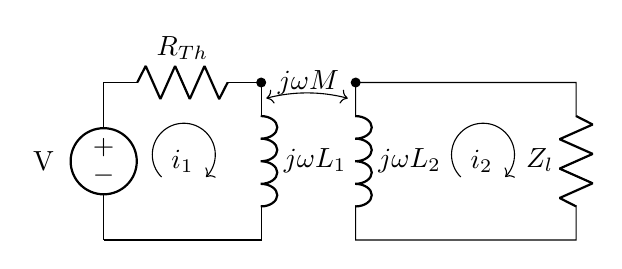
\begin{tikzpicture}[american]
\draw(0,0) to[V=V, invert] (0,2) to[resistor, R=$R_{Th}$] (2,2)
to[inductor, L=$j\omega L_1$,*-] (2,0) -- (0,0)
;
\draw(3.2,2) to [inductor,*-,L=$j\omega L_2$](3.2,0) to [short](6,0) to [resistor, R=$Z_l$](6,2) to [short](3.2,2);
\draw (1,1) node {$i_1$};
\draw[<-] (1.3,0.8) arc (-45:225:0.4);
\draw (4.8,1) node {$i_2$};
\draw[<-] (5.1,0.8) arc (-45:225:0.4);
\draw (2.6,2) node {$j\omega M$};
\draw[<->] (3.1,1.8) arc (75:105:2);


\end{tikzpicture}

$$ V_{Th}=(Z_{Th}+j\omega L_1)I_1- j\omega MI_2 $$
$$ 0 = (Z_L + j\omega L_2)I2 - j\omega MI_1$$

$$I_1= \frac{Z_L+j\omega L_2}{(Z_{Th} + j\omega L_1)(Z_L + j\omega L_2)+\omega^2M^2}V_{Th}$$
$$I_2= \frac{j\omega M}{(Z_{Th} + j\omega L_1)(Z_L + j\omega L_2)+\omega^2M^2}V_{Th}$$
$$Z_{eq}=\frac{V_{Th }}{I_1}=Z_{Th}+j\omega L_1 + \frac{\omega^2M^2}{Z_L+j\omega L_2}$$
$\frac{\omega^2M^2}{Z_L+j\omega L_2}$ is called Reflected inductance

\subsubsection{Ideal Transformer Model}

Mutual induction 
$$M=k\sqrt{L_1L_2}$$

Ideal Transformer assumptions:
\begin{itemize}
	\item Coupling coefficient $k=1$
	\item $L_1=L_2=\infty$
	\item Losses from coil resistances are negligible
\end{itemize}

add resistances on the end of the ends of the coils

$$\frac{v_1}{N_1}=\frac{v_2}{N_2}$$
$$N_1i_1=N_2i_2 $$
$N_i$ turns of the coil $i$

\subsubsection{Linear Variable Differential Transformers LVDT}
Primary coil at the "centrer" of a ferris core, the core can move.
Two secondary coils turned in opposite directions.  

if the core is on the centrer, $V_1$ and $V_2$ are complementary, the voltage across the both is approx 0

On a extreme only one secondary is linked with the primary and the output is that coil.

On an intermediate position, the amplitude is between and the phase is the coil who is fully linked. so:
\begin{itemize}
	\item Amplitude show displacement
	\item Phase shows direction
\end{itemize} 

\end{document}


